\subsubsection{Основная архитектура программной системы}
В данной работе предлагается следующая архитектура системы:
\begin{itemize}
\item модуль генерации поисковых запросов, предназначенный для обучения оценивающей части. Данный модуль предлагается
реализовать на нейросетевой основе, используя GAN-подобную архитектуру либо GPT-2;
\item поисковый модуль.
\item модуль формализации результатов, сопоставляющий каждой паре "<запрос-документ"> $\left\langle q, d \right\rangle$ набор числовых параметров
$\{p_i\}$, представляющих собой характеристики результата поискового запроса. Предлагается организовать вычисление данных характеристик на основе
классических алгоритмов без использования нейронных сетей;
\item модуль оценки релевантности, принимающий на вход набор параметров $\{p_i\}$ и выдающий результат оценки. Для данной части, представляющей 
наибольший научный и практический интерес, также предлагается использовать генеративно-состязательную нейросетевую архитектуру.
\end{itemize}
Опишем подробно каждый модуль в отдельности.

Модуль генерации поисковых запросов. Для обучения модуля оценки релевантности требуется генерировать большой объем данных (числовых векторов $\{p_i\}$),
однако, использовать случайные числа для этой цели нецелесообразно в связи с тем, что вероятностное распределение таковых может оказаться существенно
отличным от получаемого при реальных поисковых запросах. По причине того, что задача исследования распределения вероятностей требует существенного анализа,
а ручная генерация поисковых запросов в достаточных для решения основной задачи количествах технически неосуществима, более простым представляется путь 
генерации самих запросов с использованием нейронных сетей.

Данную подзадачу также возможно решать с помощью GAN-сетей, однако более перспективным представляется путь использования сети GPT-2, созданной в OpenAI.
Данная архитектура сети проектировалась авторами специально для решения задачи генерации текстов, которыми в задаче данной работы являются поисковые запросы.

Поисковый модуль. Данная часть программной системы осуществляет поиск по заданному запросу в подготовленной базе данных. В самом простом случае она
представляет собой инвертированный индекс, однако, возможно подключение, например, семантических средств (антологий, тезаурусов и т. п.) Модуль работает с
использованием классических алгоритмов, однако возможно подключение и нейронных сетей для оптимизации результатов поиска (путем хранения истории запросов
определять потенциально наиболее релевантные результаты, анализируя схожесть запросов).

Модуль формализации результатов. Служит для вычисления характеристик поискового результата (пары "<запрос-документ">), необходимых для определения его 
релевантности нейронной сетью. К числу данных характеристик, в частности, могут относиться такие параметры, как встречаемость в документе слов из запроса
либо их сочетаний, с грамматической точки зрения --- учет различных словоформ, с семантической --- учет синонимов слова в контексте запроса и т.п.
Данный модуль также реализован с использованием только классических алгоритмов, без подключения нейронных сетей.

Модуль оценки релевантности. Данная часть программной системы, как говорилось выше, представляет собой наибольший интерес, как академический, так
и практический. Здесь она реализована с помощью генеративно-состязательной сети, в которой:
\begin{itemize}
\item подсеть $G$ генерирует векторы параметров из созданных поисковых запросов на основании расчета их модулем формализации. Обучение подсети осуществляется
с помощью обратной связи от подсети $D$;
\item в свою очередь, подсеть $D$ отбирает релевантные результаты путем сравнения с базой данных заведомо релевантных запросов. В качестве источника таковых,
помимо ручного отбора результатов, представляет интерес смешанный подход, в котором определенная доля эталонов генерируется с помощью классических функций
оценки релевантности (BM25 и т.п.). Данный метод позволяет увеличить используемую выборку без повышения трудозатрат на ручную обработку, однако вопрос
качества получаемых результатов требует дальнейшего исследования.
\end{itemize}
После обучения модель пригодна к использованию для произвольных запросов, что позволяет субъективно оценить получаемые результаты.

\subsubsection{Источники текстовых документов}
В качестве корпуса текстов в реализации был использован набор данных "<Гутенберг"> (Gutenberg Dataset) ~\cite{lahiri:2014:SRW}. 
Он представляет собой собрание из 3036 книг, написанных (на английском языке) 142 авторами, преимущественно 19 века. 
Набор данных состоит из простых текстовых файлов, очищенных от любых метаданных, лицензионной информации и заметок переписчиков, 
насколько это возможно. Данные условие облегчают анализ текстов, так как позволяют избавиться от стадий предварительной обработки
и тем самым упростить задачу обучения нейросетей на текстах.

\subsubsection{База данных}
База данных была реализована с использованием СУБД ClickHouse, разработанного отечественной компанией "<Яндекс">
\cite{Clickhouse2020}. Данная СУБД обеспечивает быстрые запросы выборки (SELECT) по таблицам с большим (величиной порядка $10^9$)
количеством строк, что очень важно для решения поставленной задачи. С другой стороны, ClickHouse не подходит ни для запросов
обновления/удаления (UPDATE и DELETE), ни для "<тяжелых"> объединяющих запросов (JOIN). Однако данный факт 
не вносит большого вклада в реализацию, поскольку база слабо реляционна по своей природе. Таким образом, использование 
ClickHouse в качестве хранилища является разумным выбором.

Тексты были предварительно проанализированы с помощью лексического анализатора Penn Treebank~\cite{10.3115/1075812.1075835}
для разбора слов. Впоследствии слова были обработаны стеммером Портера~\cite{Porter1980AnAF}, чтобы восстановить основы слов, 
объединив в одной записи всевозможные грамматические формы одного слова.
Каждой основе слова, встречающемуся в текстовом корпусе, был присвоен числовой идентификатор, а идентификаторы 
с соответствующими основами хранились в SQL-таблице.

Инвертированный индекс в базе данных хранится в следующей форме (DDL-запрос):

\begin{verbatim}
    CREATE TABLE default.inv_index
    (
        `word_id` Int32,
        `document_id` Int32,
        `start_pos` Int32,
        `end_pos` Int32
    )
    ENGINE = MergeTree()
    PARTITION BY document_id
    ORDER BY document_id
    SETTINGS index_granularity = 8192
\end{verbatim}

Таким образом, таблица секционируется (разбивается на разделы-"<партиции">) по идентификатору документа, чтобы разрешить
более быстрые запросы \texttt{SELECT}, связанные с одним документом (что часто происходит при выполнении поиска).

Инвертированные индексы для биграмм и триграмм используют в основном ту же структуру, за исключением нескольких столбцов
\texttt{word\_id}.

Еще одна особенность ClickHouse, которая широко используется здесь, --- это возможность создавать материализованные представления.
Это в основном представления SQL с кэшированным результатом, хранящимся на диске. Они особенно полезны, например, при запросе
количества слов в документе (чтение кэшированных данных дает значительное, иногда на порядок, ускорение).

\subsubsection{Генерация поисковых запросов}
Генератор запросов основан на реализации сети GPT-2 с помощью Python-пакета \texttt{textgenrnn}~\cite{TextgenRNN2020}. Данная 
реализация написана с использованием фреймворка Keras~\cite{chollet2015keras}. На более низком уровне используется библиотека
TensorFlow~\cite{tensorflow2015-whitepaper}, в которой для ускорения обучения сети путем расчетов на графическом процессоре
применяется cuDNN~\cite{DBLP:journals/corr/ChetlurWVCTCS14} --- библиотека, разработанная компанией nVIDIA специально для 
обучения нейронных сетей с помощью CUDA~\cite{cuda}. Топология сети в пакете \texttt{textgenrnn} представлена на рис.~\ref{fig:default}

\begin{figure}
    \centerline{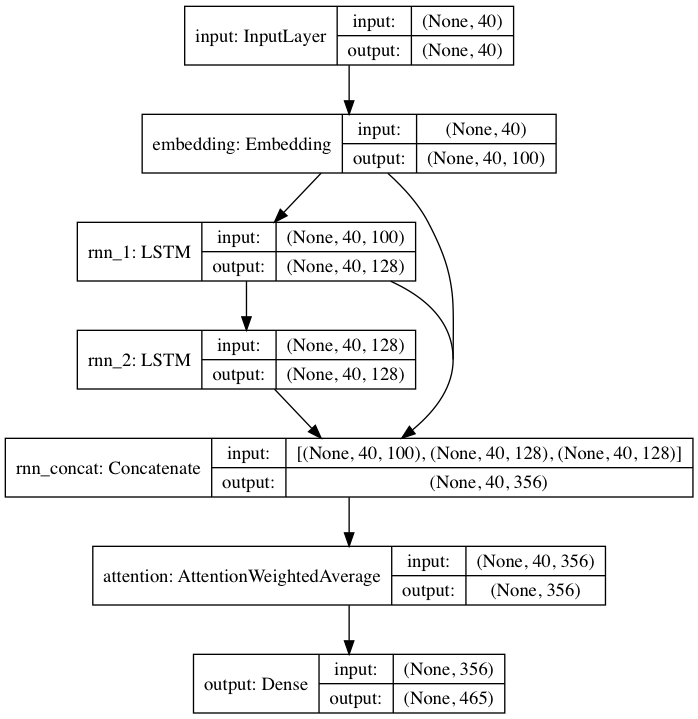
\includegraphics[scale=0.5]{default_model.png}}
    \caption{Структура модели нейронной сети в \texttt{textgenrnn}}\label{fig:default}
\end{figure}

Чтобы сгенерированные запросы были потенциально релевантны пространству поиска, сеть GPT-2 должна быть обучена на одном и том же
наборе текстов. Чтобы избежать более длительного времени обучения, но вместе с тем сохранить качество и отношение к предметной области,
для обучения рекуррентной сети была выбрана доля набора данных в размере 5\% (всего 152 документа и около 13 миллионов слов).

Кроме того, чтобы результирующие запросы не были слишком универсальными (например, содержащими только "<стоп-слова">, такие как
артикли, предлоги и другие часто используемые слова), на генератор накладываются некоторые ограничения. А именно, запрос считается
"<хорошим"> тогда и только тогда, когда он удовлетворяет одному из следующих условий:

\begin{enumerate}[1)]
    \item как минимум 1 слово встречается не более чем в 25\% от всех документов из коллекции;
    \item как минимум \(\frac{1}{3}\) слов (с округлением до ближайшего целого числа) встречается
    не более чем в 40\% от всех документов из коллекции.
\end{enumerate}

В общей сложности, в качестве эталонных было выбрано 242 запроса (на английском языке).

Примеры сгенерированных запросов:
\begin{itemize}
    \item \textit{returned earl   we had }
    \item \textit{trouble to move in oz mode which}
    \item \textit{and i don really want you to take}
    \item \textit{literature seems to be the loveliest ends }
    \item \textit{your distinction  it is i cannot as}
\end{itemize}

Как видим (по крайней мере, с точки зрения неносителя языка), запросы вполне сходны по структуре с "<настоящими"> поисковыми
запросами к системам общего назначения, таким, как Google.

Далее, в качестве эталона псевдорелевантности для обучения нейронной сети были отобраны по 10 верхних результатов по каждому из
запросов. Результаты были отранжированы согласно модифициорванной формуле BM25:
\begin{equation}
    \label{eq:wbm25}
    \begin{aligned}
    \text{score}(D,Q) = w_1 \sum_{i=1}^{n} \text{IDF}(q_i) \times \\ \times \frac{f(q_i, D) \cdot (k_1 + 1)}{f(q_i, D) + k_1 \cdot \left(1 - b + b \cdot \frac{|D|}{\tilde{L}}\right)} \\
    + w_2  \sum_{i=1}^{n-1} \text{IDF}(q_i q_{i+1}) \times \\ \times \frac{f(q_i q_{i+1}, D) \cdot (k_1 + 1)}{f(q_i q_{i+1}, D) + k_1 \cdot \left(1 - b + b \cdot \frac{|D| - 1}{\tilde{L} - 1}\right)} \\
    + w_3  \sum_{i=1}^{n-2} \text{IDF}(q_i q_{i+1}q_{i+2}) \times \\ \times \frac{f(q_i q_{i+1}q_{i+2}, D) \cdot (k_1 + 1)}{f(q_i q_{i+1}q_{i+2}, D) + k_1 \cdot \left(1 - b + b \cdot \frac{|D| - 2}{\tilde{L} - 2}\right)}
    \end{aligned}
\end{equation}
где \(w_1\), \(w_2\), \(w_3\) --- весовые коэффициенты отдельных слов, биграмм и триграмм соответственно (в реализации 
использовались значения \(w_1=1\), \(w_2=10\) and \(w_3=100\)), \(f(q_1, D)\), \(f(q_1q_2, D)\) и \(f(q_1q_2q_3, D)\) --- 
частоты терминов: отдельного слова \(q_1\), биграммы \(q_1q_2\) и триграммы \(q_1q_2q_3\) соответственно (аналогично и для IDF),
 \(|D|\) --- длина документа \(D\), а \(\tilde{L}\) --- средняя длина документа в коллекции (слагаемые \(-1\) and \(-2\) 
для биграмм и триграмм соответственно были введены в связи с тем, что документ с \(N\) словами, очевидно, содержит 
\(N-1\) биграмму и \(N-2\) триграммы, поэтому "<длина"> документа окажется на один и два меньше соответственно).

Таким образом, эталонный набор данных включал в себя 2158 результатов
(это число меньше, чем $10\times242=2420$, поскольку некоторые запросы дали менее 10 результатов в целом).

\subsubsection{Генеративно-состязательная сеть}
GAN-сеть состояла из следующих подсетей:
\begin{itemize}
    \item подсеть $G$, использующая случайные 100-мерные векторы в качестве входных данных 
    и 32-мерные векторы результатов (метрик) запроса в качестве выходных данных;
    \item подсеть $D$, которая принимает 32-мерные векторы (как порожденные подсетью $G$, так и эталонные) и выводит скаляр, 
    который может быть интерпретирован как "<вероятность"> того, что запрос является псевдорелевантным.
\end{itemize}

В сети использовались следующие функции активации:
\begin{itemize}
    \item гиперболический тангенс
    \begin{equation}
        f(x) = \tanh x;
    \end{equation}
    \item сигмоида
    \begin{equation}
        f(x) = \frac{1}{1+e^{-x}};
    \end{equation}
    \item выпрямитель с "<протечкой"> ~\cite{DBLP:journals/corr/XuWCL15} (leaky rectified linear unit)
    \begin{equation}
        f(x) = \begin{cases}
            x, & x \geqslant 0, \\
            \alpha x, & x < 0.
        \end{cases}
    \end{equation}
\end{itemize}

Внутри подсети $G$ используется последовательное размещение слоев, как показано ниже:
\begin{itemize}
    \item входной слой с размером 100 (для случайного
    входа);
    \item слой с 256 нейронами, с использованием выпрямителя с протечкой при $\alpha = 0.2$;
    \item слой с 512 нейронами, с использованием выпрямителя с протечкой при $\alpha = 0.2$;
    \item слой с 1024 нейронами, с использованием выпрямителя с протечкой при $\alpha = 0.2$;
    \item выходной слой с размером 32, использующий гиперболический тангенс в качестве функции активации.
\end{itemize}
Внутри подсети $D$ также используется последовательное размещение слоев в следующем порядке:
\begin{itemize}
    \item входной слой с размером 32 (для подачи векторов параметров, генерируемых подсетью G);
    \item слой с 1024 нейронами, использующий ReLU с $\alpha = 0.2$;
    \item слой отсева с коэффициентом 0,3;
    \item слой с 512 нейронами, использующий ReLU с $\alpha = 0.2$;
    \item слой отсева с коэффициентом 0,3;
    \item слой с 256 нейронами, использующий ReLU с $\alpha = 0.2$;
    \item слой отсева с коэффициентом 0,3;
    \item выходной слой с размерностью 1 (скалярное значение, обозначающее оценку релевантности).
\end{itemize}

Для проверки сгенерированной модели был сгенерирован дополнительный набор из 51 "<хорошего"> запроса. Затем 
было использовано классическое ранжирование BM25 по формуле \eqref{eq:wbm25}, после чего из результатов поиска 
по каждому запросу были выделены верхние 10 (псевдорелевантные) и нижние 10 (псевдонерелевантные).
На следующем этапе результаты подавались через обученную модель. Некоторые результаты приведены в таблице \ref{tab1}
(средние значения $\mu$ и стандартные отклонения $\sigma$ оценок GAN-сетью для верхней и нижней групп 10).

\begin{table}[tbp]
    \caption{Результаты поисковых запросов}
    \begin{center}
    \begin{tabular}{ccc}
    \toprule
    \textbf{Запрос}&\multicolumn{2}{c}{\textbf{Оценка релевантности}} \\
    & \textbf{\textit{Top 10}}& \textbf{\textit{Bottom 10}} \\
    \midrule
    that there were no reason on lewis& \(\mu=0.8024\) & \(\mu=0.6926\) \\
    & \(\sigma=0.1050\) & \(\sigma=0.0474\) \\
    \midrule
    i proposed marriage his visit& \(\mu=0.5127\) & \(\mu=0.1933\) \\
    & \(\sigma=0.2786\) & \(\sigma=0.0694\) \\
    \midrule
    fanny  said she& \(\mu=0.7270\) & \(\mu=0.2061\) \\
    & \(\sigma=0.2269\) & \(\sigma=0.0086\) \\
    \midrule
    published it  i think we found& \(\mu=0.2096\) & \(\mu=0.0822\) \\
    & \(\sigma=0.2077\) & \(\sigma=0.0226\) \\
    \midrule
    i shall you heart now & \(\mu=0.4713\) & \(\mu=0.1577\) \\
    & \(\sigma=0.3046\) & \(\sigma=0.0095\) \\
    \midrule
    right i had down her & \(\mu=0.4439\) & \(\mu=0.1843\) \\
    & \(\sigma=0.1391\) & \(\sigma=0.0985\) \\
    \midrule
    nice declaration  she got you  i & \(\mu=0.7382\) & \(\mu=0.3731\) \\
    & \(\sigma=0.2437\) & \(\sigma=0.0203\) \\
    \midrule
    i never moved nearer than it is & \(\mu=0.7801\) & \(\mu=0.2660\) \\
    & \(\sigma=0.1304\) & \(\sigma=0.2241\) \\
    \bottomrule
    \end{tabular}\label{tab1}
    \end{center}
\end{table}